\documentclass[a4paper, 12pt]{article}
\usepackage[top=2cm, bottom=2cm, left=1.5cm, right=1.5cm]{geometry}
\usepackage[utf8]{inputenc}
\usepackage{amsmath, amsfonts, amssymb}
\usepackage{graphicx}
\usepackage{float}
\usepackage{indentfirst}
\usepackage[small,bf]{caption}
\newcommand{\PR}[1]{\ensuremath{\left[#1\right]}} %Para exemplo muito rápido, se a intenção for colocar \displaystyle \frac{1}{2} entre parênteses curvos então escrevo: \PC{\frac{1}{2}}
\newcommand{\PC}[1]{\ensuremath{\left(#1\right)}}
\newcommand{\chav}[1]{\ensuremath{\left\{#1\right\}}}


\begin{document}
%%%%%%%%%%%%%%%%%%%%%%%%%%%%%%%%Começo do documento%%%%%%%%%%%%%%%%%%%%%%%%

\begin{center}
Nome:\_\_\_\_\_\_\_\_\_\_\_\_\_\_\_\_\_\_\_\_\_\_\_\_\_\_\_\_\_\_\_\_\_\_\_\_\_\_\_\_\_\_\_\_\_\_\_\_\_\_\_\_\_\_\_\_\_\_\_\_\_\_\_\_ \hspace{3cm} Data: \_\_ / \_\_ / $2019$
\end{center}

\vspace{0.07 cm}

\begin{center}
	\begin{Large}
	\textbf{PROCEU - Prova de conhecimentos básicos}
	\end{Large}
\end{center}
			

\vspace{0.07 cm}
	
	
	\begin{enumerate}
	
	\item Determine o valor da expressão:
	$$ 2 + 3 \cdot \chav{5 - 3 \cdot \PR{ 11 + 5 - 2 \cdot \PC{\frac{9}{3} + 5 + 2^3 + 5 \cdot 7} + 6 } -18 } + 3^3  .$$
\vspace{0.01cm}

	
	\item Em uma cidade do interior de São Paulo, $30\%$ dos habitantes têm menos de 20 anos, $55\%$ dos habitantes tem entre 20 e 60 anos, e o restante tem mais de 60 anos. Dado que a cidade tem $500.000$ habitantes, qual o número de pessoas que tem mais de 60 anos?
\vspace{0.7cm}	
	
	
	
	
	\item Petrônio decidiu viajar de férias, e saiu de casa com o tanque do carro cheio. Sabe-se que ele já percorreu $\frac{1}{4}$ do caminho, gastando $\frac{3}{4}$ do tanque de combustível. Quantas paradas para abastecimento serão necessárias para que Petrônio chegue a seu destino?
\vspace{0.7cm}
	
	
	
	
	\item Os logaritmos possuem várias aplicações na Matemática e em diversas áreas do conhecimento, como Física, Biologia, Química, Medicina, Geografia, entre outras. Definimos logaritmo como sendo o expoente que se deve elevar uma base, de modo que o resultado seja uma determinada potência. Isto é:

			$$ \log_a b = x \Longleftrightarrow b = a^x $$

Onde $a$ é a \textit{base}, $b$ o \textit{logaritmando} e $x$ o \textit{logaritmo}. Com $a$ e $b$ positivos e $a \neq 1$. \\

Devido às suas propriedades, o uso de logaritmos facilita cálculos que envolvem números muito grandes ou pequenos. Algumas dessas propriedades são: \textit{logaritmo do produto}, \textit{logaritmo do quociente} e \textit{logaritmo da potência}. Com isso, pede-se para calcular os seguintes valores de logaritmo:

		\begin{enumerate}
   		 \item $\log_{10}6$ sabendo que $\log_{10} 2 = 0,30$ e $\log_{10} 3 = 0,47$.
    
    		\item $\log_{10}4$ sabendo que $4 = 2^2$.
    
    		\item $\log_{10} \PC{ \dfrac{5}{4} }$ sabendo que o $\log_{10} 5 = 0,69$
\end{enumerate} 
\vspace{0.7cm}





	\item Maria está fazendo uma reforma em sua casa e contratou 7 pedreiros. Com este número de trabalhadores, Maria gastará no total R\$ $52.500,00$ para pagar seus salários.
	\begin{enumerate}	
    	\item Quanto gastaria Maria caso tivesse contratado 10 pedreiros?
    	\item Se os 7 pedreiros reformam a casa em 33 dias, quantos pedreiros seriam necessários para terminá-la em 21 dias?
	\end{enumerate}
%\vspace{0.7cm}
\pagebreak
 
 
 
	\item O Teorema de Pitágoras nos diz que um triângulo possui um ângulo reto se, e só se, existe uma relação entre seus lados tal que $a^2 = b^2 + c^2$ (vide figura abaixo).
		
		\begin{figure}[h]
		\centering
		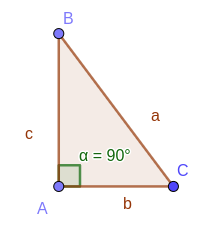
\includegraphics[scale = 0.60]{triangulo}
		%\caption{}
		\end{figure}
		
	 Os lados de um dado triângulo $ABC$ medem $10 \, cm$, $24 \, cm$ e $26 \, cm$. É possível afirmar que esse é um triângulo retângulo? Justifique.
\vspace{0.7cm}


	
	\item Uma empresa registrou seu desempenho em determinado ano por meio de um gráfico, com dados mensais do total de vendas e despesas.
		\begin{figure}[!h]
		\centering
		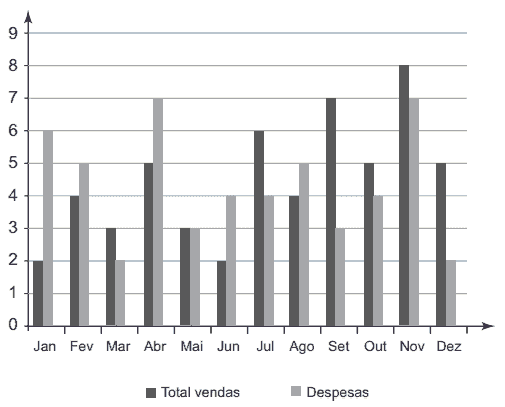
\includegraphics[scale = 0.40]{grafico}
		%\caption{}
		\end{figure}
			
O lucro mensal é obtido pela subtração entre o total de vendas e despesas, nesta ordem. Dizemos que houve prejuízo se o valor das despesas for superior ao total de vendas. Qual o mês do ano em que foi registrado o maior lucro? E o pior prejuízo? Em qual mês o lucro foi igual a zero?
\vspace{0.7cm}



	\item Dado o prisma a seguir, determine:
		
		\begin{minipage}{.5\linewidth}		
			\begin{figure}[H]
			\centering
			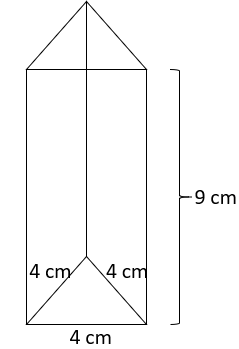
\includegraphics[scale= 0.5]{prisma}
			\end{figure}
		\end{minipage}
		\begin{minipage}{.5\linewidth}		
			\begin{enumerate}
				\item O volume do prisma regular de base triangular
				\item A área lateral
				\item A área total
			\end{enumerate}	
		\end{minipage}\\

		
Adote: área da base triangular como sendo $4\sqrt{3} \, cm^2$ e a altura do prisma igual a $9 \, cm$.
\vspace{0.7cm}
	
	
	
	\end{enumerate}	

%%%%%%%%%%%%%%%%%%%%%%%%%%%%%%%%%%%%%%%%%%%%%%%%%%%%%%%%%%%%%%%%%%%%%%%%
\end{document}